%
% teil2.tex -- Beispiel-File für teil2 
%
% (c) 2020 Prof Dr Andreas Müller, Hochschule Rapperswil
%
\section{Das Zuordnungsproblem
\label{munkres:section:teil2}}
\rhead{Das Zuordnungsproblem}
Das (lineare) Zuordnungsproblem ist ein diskretes Optimierungsproblem aus
der Graphentheorie.
Es handelt sich um einen Spezialfall eines maximalen Matchings
minimalen Gewichtes in einem bipartiten, gewichteten Graphen

Vereinfacht gesagt sind Zuordnungsprobleme spezielle Transportprobleme.
Der Unterschied zu klassischen Transportproblemen liegen darin,
dass hier nicht Mengen möglichst kostenminimal von einem zum anderen
Ort transportiert werden sollen, sondern es geht um die kostenminimale
Zuordnung von z.~B.~Personen, oder Bau-Materialien auf bestimmte
Orte, Stellen oder Aufgaben.
Dabei sind alle Angebots- und Bedarfsmenge gleich 1 
\begin{equation}
a_{i}=b_{j}=1
\end{equation}

\subsection{Zuordnungsproblem in Netzwerkdarstellung
\label{munkres:subsection:bonorum}}

\begin{figure}
\centering
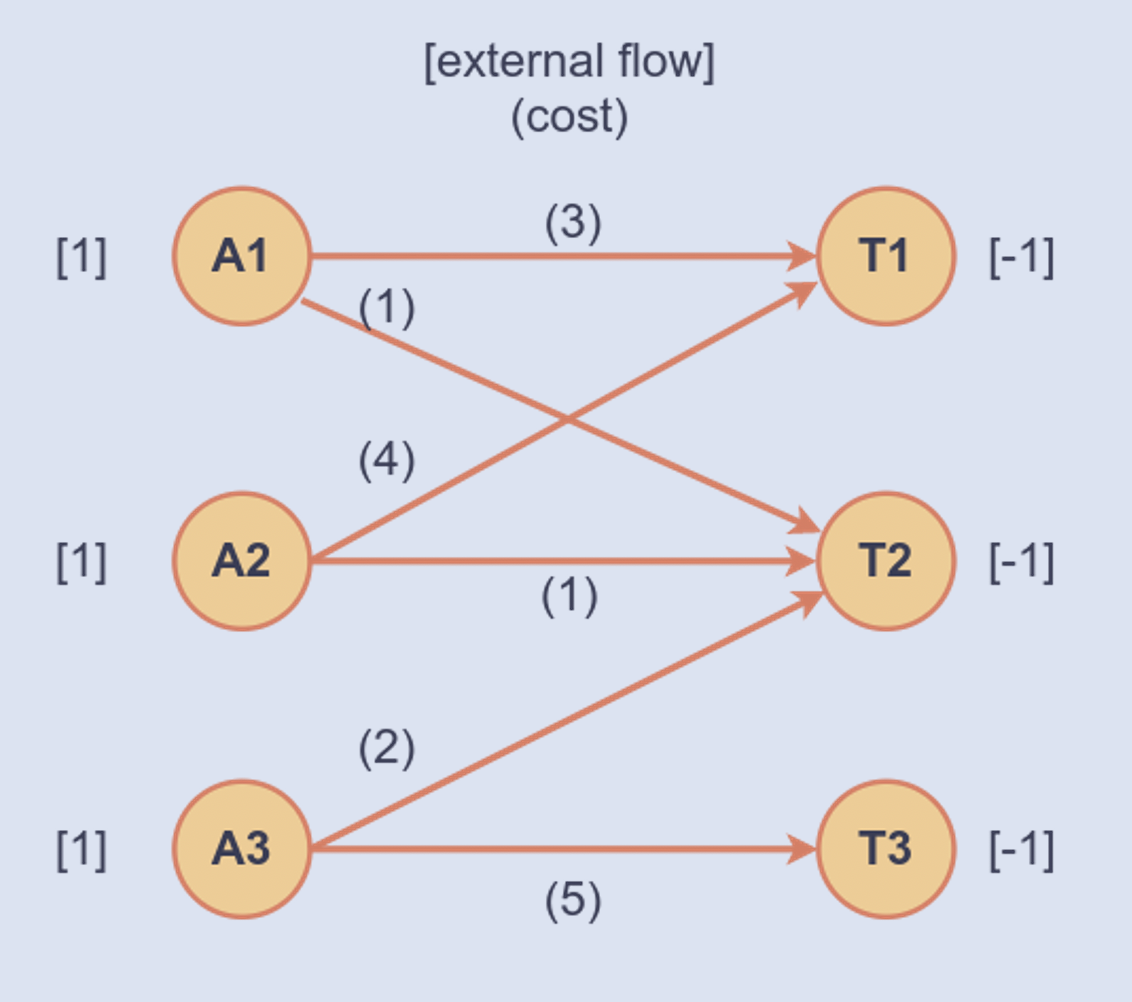
\includegraphics[width=5cm]{papers/munkres/figures/Netzwerkdarstellung}
\caption{Typische Netzwerkdarstellung eines Zuordnungsproblems.}
\label{munkres:Vr2}
\end{figure}

\subsection{Matrix Formulierung
\label{munkres:subsection:bonorum}}
In der Matrixformulierung ist eine nicht-negative $n\times n$-Matrix
gegeben, wobei das Element in der $i$-ten Zeile und $j$-ten Spalte
die Kosten für die Zuweisung des $j$-ten Jobs an den $i$-ten Arbeiter
darstellt.
Wir müssen eine Zuordnung der Jobs zu den Arbeitern finden, so dass
jeder Job einem Arbeiter zugewiesen wird und jeder Arbeiter einen
Job zugewiesen bekommt, so dass die Gesamtkosten der Zuordnung
minimal sind.
Dies kann als Permutation der Zeilen und Spalten einer Kostenmatrix
$C$ ausgedrückt werden, um die Spur einer Matrix zu minimieren:
\begin{equation}
\min(L,R)Tr (LCR)
\end{equation}
wobei $L$ und $R$ Permutationsmatrizen sind.
Wenn das Ziel ist, die Zuordnung zu finden, die die maximalen Kosten
ergibt, kann das Problem durch Negieren der Kostenmatrix $C$ gelöst
werden.

\subsection{Suche der optimalen Lösung
\label{munkres:subsection:bonorum}}
Ist eine maximale Zuordnung (maximales Matching) gefunden, so steht
in jeder Zeile und jeder Spalte der Matrix genau ein Element, das
zur optimalen Lösung gehört, eine solche Gruppe von Positionen wird
auch als Transversale der Matrix bezeichnet.
Deshalb kann die Problemstellung auch anders formuliert werden: Man
ordne die Zeilen- oder die Spaltenvektoren so um, dass die Summe
der Elemente in der Hauptdiagonale maximal wird.
Hieraus wird sofort ersichtlich, dass es in einer 
$n\times n$-Matrix genau so viele Möglichkeiten gibt, die Zeilen-
bzw.~Spaltenvektoren zu ordnen, wie es Permutationen von $n$ Elementen
gibt, also $n!$.
Außer bei kleinen Matrizen ist es nahezu aussichtslos, die optimale
Lösung durch Berechnung aller Möglichkeiten zu finden.
Schon bei einer $10\times 10$-Matrix gibt es nahezu 3,63 Millionen (3.628.800)
zu berücksichtigender Permutationen.

\subsection{Formulierung Bipartiter Graph
\label{munkres:subsection:bonorum}}
Der Algorithmus ist einfacher zu beschreiben, wenn wir das Problem
anhand eines bipartiten Graphen formulieren.
Wir haben einen vollständigen zweistufigen Graphen $G=(S,T;E)$ mit
$n$ Arbeiter-Eckpunkten ($S$) und $n$ Job-Scheitelpunkte ($T$), und
jede Kante hat einen nichtnegativen Preis $c(i,j)$.
Wir wollen ein perfektes Matching mit minimalen Gesamtkosten finden.

\begin{figure}
\centering
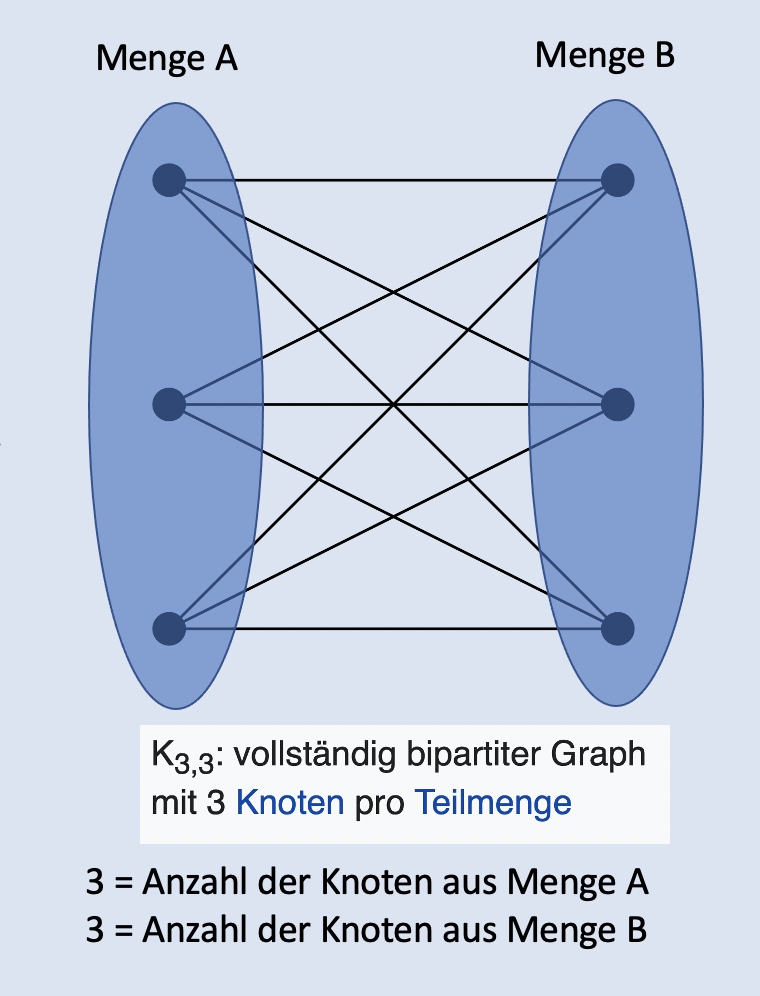
\includegraphics[width=5cm]{papers/munkres/figures/bipartiter_graph}
\caption{$K_{3,3}$ vollständig bipartiter Graph mit 3 Knoten pro Teilmenge.}
\label{munkres:Vr2}
\end{figure}

